   
\documentclass[11pt, answers]{exam}
\renewcommand{\baselinestretch}{1.05}
\usepackage{amsmath,amsthm,verbatim,amssymb,amsfonts,amscd, graphicx}
\usepackage{graphics}

\usepackage{afterpage}
\usepackage{caption}

\usepackage{tikz}
\usepackage{fancybox}

\usepackage{clrscode3e}

\topmargin0.0cm
\headheight0.0cm
\headsep0.0cm
\oddsidemargin0.0cm
\textheight23.0cm
\textwidth16.5cm
\footskip1.0cm
\theoremstyle{plain}
\newtheorem{theorem}{Theorem}
\newtheorem{corollary}{Corollary}
\newtheorem{lemma}{Lemma}
\newtheorem{proposition}{Proposition}
\newtheorem*{surfacecor}{Corollary 1}
\newtheorem{conjecture}{Conjecture}  
\theoremstyle{definition}
\newtheorem{definition}{Definition}

 \begin{document}
 


\title{CSC265: Assignment 1}
\author{Ruo yi Lin and Junjie Cheng}
\maketitle

\unframedsolutions

\begin{questions}

\question

\begin{parts}

\part Describe in detail a data structure implementing the Partial-Sums ADT. Draw an example with $n=8$, and values $a_1,\ldots,a_8$ of your choosing, but not $a_1=\ldots=a_8=0$. \\

\begin{solution}
The correct data structure is a full binary tree of height $k, B_k$. There are $2^k = n$ leaves in the lowest row of this tree. The $i$th leaf holds value $a_i$. The values of the parent nodes are defined recursively as the sum of their two children. An example is below with $a_1, \ldots, a_n = 1, 2, 3, 4, 5, 6, 7, 0$.
\\


\begin{center}
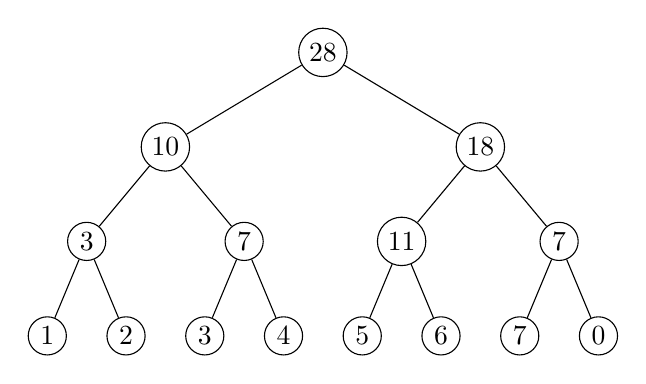
\begin{tikzpicture} 
[ 
level distance=12mm, 
every node/.style={circle, draw, inner sep=2pt},
level 1/.style={sibling distance=40mm}, 
level 2/.style={sibling distance=20mm}, 
level 3/.style={sibling distance=10mm}
]

\node {28} 
child {node {10} 
	child {node {3} 
		child {node {1}} 
		child {node {2}}
	}
	child {node {7} 
		child {node {3}} 
		child {node {4}}
	} 
}
child {node {18}
 	child {node {11} 
 		child {node {5}} 
 		child {node {6}}
 	}
 	child {node {7}
		child {node {7}}
		child {node {0}}
	}
};	 
\end{tikzpicture}
\end{center}

\end{solution}

\part Describe in clear and precise English how to implement the three operations $\proc{Init}$, $\proc{Add}(i,t)$, and $\proc{Sum}(i)$. Give pseudocode for $\proc{Add}(i,t)$, and $\proc{Sum}(i)$. For each operation argue why it computes the correct output, and show that it runs in the required worst-case running time.

\begin{itemize}
\item $\proc{Init}$ must run in time $\func{O}(n)$
\item $\proc{Add}(i,t)$ must run in time $\func{O}(\log(n))$
\item $\proc{Sum}(i)$ must run in time $\func{O}(\log(n))$
\end{itemize}

\begin{solution}\\

$\proc{Init}$:
Since $n = 2^k$, the binary tree required by the Partial-Sums ADT will always be full. Then the tree can be easily implemented as an array of size $2^{k+1} - 1$, with initial values all set to $0$. We assume that the first index of the array is $1$.

There is no need to construct pointers, since for a complete binary tree there are simple closed-form expressions for parent and child nodes. The functions are reproduced from CLRS Section 6.1.

Then $\proc{Init}$ runs in time $\func{O}(2^{k+1} - 1) = \func{O}(2(2^k)) = \func{O}(2n) = \func{O}(n)$.

\begin{codebox}
\Procname{$ \proc{Parent}(i)$}
\li 		\Return $\lfloor i/2 \rfloor$
\end{codebox}

\begin{codebox}
\Procname{$ \proc{Left-Child}(i)$}
\li 		\Return $2i$
\end{codebox}

\begin{codebox}
\Procname{$ \proc{Right-Child}(i)$}
\li 		\Return $2i + 1$
\end{codebox}

$\proc{Add}(i,t)$:
Add is simple to implement. The $i$th leaf of the tree is given by index $2^k + i$. We add $t$ to this leaf, and then add $t$ to each of $i$'s parents, grandparents, great-grandparents $\ldots$ until we reach the root.

\begin{codebox}
\Procname{$\proc{Add}(i,t)$}
\li $\func{node\_index} \gets 2^k + i$
\li \While $\func{node\_index} \neq 0$
\li \Do $\func{node\_index.value} \gets \func{node\_index.value} + t$
\li $\func{node\_index} = \proc{Parent}(\func{node\_index})$
\End
\end{codebox}

The resultant tree has an updated leaf and satisfies the sum property specified in $\proc{Init}$. This is because only the parents of the leaf specified by $i$ will have their values affected.

$\proc{Add}(i,t)$ runs in $\func{O}(\log(n))$. One iteration of the while loop is executed for each level of the tree, so the algorithm is proportional to the tree height. This in turn is proportional to the log of the number of nodes in the tree, which is proportional to the number of leaves. \\

We may reach the same conclusion by noticing that $\func{node\_index}$ is proportional to $n$ and that it is halved on each iteration when $\proc{Parent}$ is called.
\\

$\proc{Sum}(i)$:
Notice that for any node $N$ at depth $h$ of the tree, there are $2^{n-h}$ descendants of $N$ which are leaves. We can show by induction that the value contained in $N$ is equal to the sum of its leaf descendants. This is key to our algorithm. We start by initializing a running sum variable, $x$, at zero. Then we traverse the tree downwards from the root, choosing at each depth $h$ at most one node $N$. We add the value of $N$ to our running sum $x$. Our choice of $N$ is based on the value of $i$, so that

\begin{enumerate}
\item No value $a_j$ ($1 \leq j \leq n$) is added more than once
\item The algorithm terminates once $x$ contains the sum $a_1, \ldots, a_i$
\end{enumerate}

Since we can represent $i$ uniquely in binary, we can decompose it into a unique sum of these "power of two" nodes. Since the algorithm chooses and adds only a single node at each depth $h$ of a tree, it runs in $\func{O}(\log(n))$ time.

An example of the algorithm is illustrated with $i = 7, n = 8$. Our pseudocode is less intuitive, because it uses the array-index implementation of a complete binary tree (given in CLRS 6.1). The first index in the array is 1. 

\begin{minipage}[t]{\linewidth}
                \centering
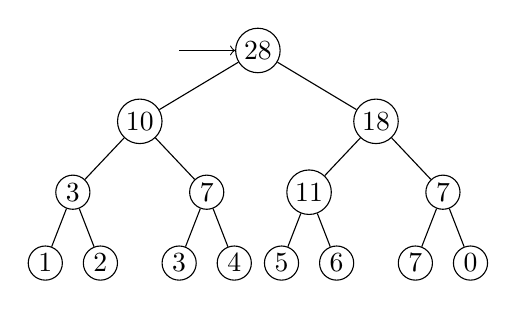
\begin{tikzpicture}
[ 
level distance=9mm, 
every node/.style={circle, draw, inner sep=1.5pt},
level 1/.style={sibling distance=30mm}, 
level 2/.style={sibling distance=17mm}, 
level 3/.style={sibling distance=7mm}
]

\node (root) {28} 
child {node {10} 
	child {node {3} 
		child {node {1}} 
		child {node {2}}
	}
	child {node {7} 
		child {node {3}} 
		child {node {4}}
	} 
}
child {node {18}
 	child {node {11} 
 		child {node {5}} 
 		child {node {6}}
 	}
 	child {node {7}
		child {node {7}}
		child {node {0}}
	}
};
\coordinate[left of=root] (invisi);
\draw[->] (invisi) -- (root);
\end{tikzpicture}
\end{minipage}

\begin{minipage}[t]{\linewidth}
                \centering
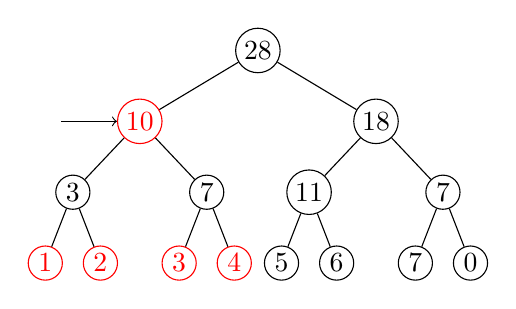
\begin{tikzpicture}
[ 
level distance=9mm, 
every node/.style={circle, draw, inner sep=1.5pt},
level 1/.style={sibling distance=30mm}, 
level 2/.style={sibling distance=17mm}, 
level 3/.style={sibling distance=7mm}
]

\node (root) {28} 
child {node[red] (hey) {10} 
	child {node {3} 
		child {node[red] {1}} 
		child {node[red] {2}}
	}
	child {node {7} 
		child {node[red] {3}} 
		child {node[red] {4}}
	} 
}
child {node {18}
 	child {node {11} 
 		child {node {5}} 
 		child {node {6}}
 	}
 	child {node {7}
		child {node {7}}
		child {node {0}}
	}
};
\coordinate[left of=hey] (invisi);
\draw[->] (invisi) -- (hey);
\end{tikzpicture}
\end{minipage}

\begin{minipage}[t]{\linewidth}
                \centering
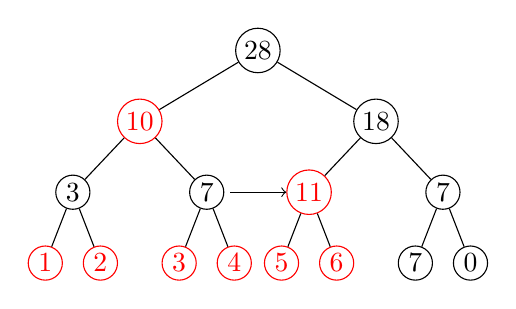
\begin{tikzpicture}
[ 
level distance=9mm, 
every node/.style={circle, draw, inner sep=1.5pt},
level 1/.style={sibling distance=30mm}, 
level 2/.style={sibling distance=17mm}, 
level 3/.style={sibling distance=7mm}
]

\node (root) {28} 
child {node[red] (hey) {10} 
	child {node {3} 
		child {node[red] {1}} 
		child {node[red] {2}}
	}
	child {node {7} 
		child {node[red] {3}} 
		child {node[red] {4}}
	} 
}
child {node {18}
 	child {node[red] (hey2) {11} 
 		child {node[red] {5}} 
 		child {node[red] {6}}
 	}
 	child {node {7}
		child {node {7}}
		child {node {0}}
	}
};
\coordinate[left of=hey2] (invisi);
\draw[->] (invisi) -- (hey2);
\end{tikzpicture}
\end{minipage}

\begin{minipage}[t]{\linewidth}
                \centering
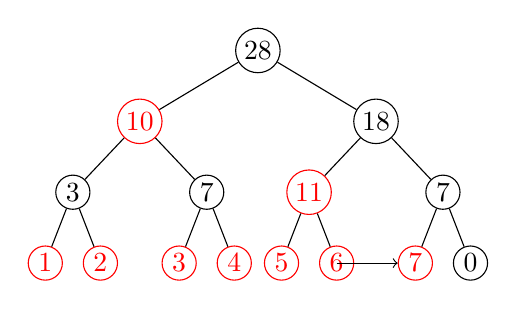
\begin{tikzpicture}
[ 
level distance=9mm, 
every node/.style={circle, draw, inner sep=1.5pt},
level 1/.style={sibling distance=30mm}, 
level 2/.style={sibling distance=17mm}, 
level 3/.style={sibling distance=7mm}
]

\node (root) {28} 
child {node[red] (hey) {10} 
	child {node {3} 
		child {node[red] {1}} 
		child {node[red] {2}}
	}
	child {node {7} 
		child {node[red] {3}} 
		child {node[red] {4}}
	} 
}
child {node {18}
 	child {node[red] (hey2) {11} 
 		child {node[red] {5}} 
 		child {node[red] {6}}
 	}
 	child {node {7}
		child {node[red] (hey3) {7}}
		child {node {0}}
	}
};
\coordinate[left of=hey3] (invisi);
\draw[->] (invisi) -- (hey3);
\end{tikzpicture}



\end{minipage}

In the pseudocode, $i \func{div} c \gets \lfloor i / c \rfloor$ and $i \bmod c$ is the usual modulus function. $\func{value}(d)$ is a function which returns the value of the node with index $d$.



\begin{codebox}
\Procname{$\proc{Sum}(i)$}
\li $d \gets 1$
\li $b \gets i$
\li $c \gets n$
\li $x \gets 0$
\li \While $b > 0$ \Do
\li		\If $(\lfloor b / c \rfloor = 1)$ \Then
\li 		$b \gets b - c$
\li			$x \gets x + \func{value}(d)$
\li 		$d = 2d + 2$
\li		\Else
\li			$d = 2d$	
		\End
\li	$c \gets \lfloor c / 2 \rfloor$ 		
	\End
\li \Return $x$
\end{codebox}

Proof of correctness.
The following lemma essentially states that the value held by a node is equal to the sum of the values of its leaf descendants.
\begin{lemma}
If the index of a node $N$ in an array-implementation of a $\proc{Sum}$ complete binary tree of height $k$ is $2^h + \mathit{l}$, then $\func{N.value}$ is \[\sum_{j = (2^{k-h})\mathit{l} + 1}^{(2^{k-h})\mathit{l} + 2^{k-h}}a_j.\]
\end{lemma}
\begin{proof}
We fix the size of the tree, $k$, and proceed by induction \emph{up} the levels of the tree. 

\emph{Base case:} $h = k$. Fix $\mathit{l}$. Then $N$ is a leaf and 

\begin{gather*}
\sum_{j = (2^{k-h})\mathit{l} + 1}^{(2^{k-h})\mathit{l} + 2^{k-h}}a_j 
 = \sum_{j = \mathit{l} + 1}^{\mathit{l} + 1}a_j
 = a_{l + 1} = \func{N.value}
\end{gather*}

So the base case holds. Note $\mathit{l} = 0$ for the first node at depth $h$ in the tree.

\emph{Inductive Case:} Suppose that the lemma holds for all nodes at depth $h + 1$ of the tree. We show that it holds for nodes at depth $h$. Fix $\mathit{l}$.

By construction, $\func{N.value} = \func{N.left.value} + \func{N.right.value}$. The index of $\func{N.left}$ is $2(2^h + \mathit{l}) = 2^{h+1} + 2\mathit{l}$ and the index of $\func{N.right}$ is $2(2^h + \mathit{l}) + 1 = 2^{h+1} + 2\mathit{l} + 1$. We apply the induction hypothesis on the children of $N$ to obtain

\begin{gather*}
\func{N.value} = 
\sum_{j = (2^{k-(h+1)})(2 \mathit{l}) + 1}^{(2^{k-(h+1)})(2 \mathit{l}) + 2^{k-(h+1)}}a_j + 
\sum_{j = (2^{k-(h+1)})(2 \mathit{l} + 1) + 1}^{(2^{k-(h+1)})(2 \mathit{l} + 1) + 2^{k-(h + 1)}}a_j \\
= \sum_{j = (2^{k-h}) \mathit{l} + 1}^{(2^{k-h)})\mathit{l} + 2^{k-(h+1)}}a_j + 
\sum_{j = (2^{k-h})\mathit{l} + 2^{k-h} + 1}^{(2^{k-h}) \mathit{l} + (2^{k-(h + 1)}) + 2^{k-(h + 1)}}a_j \\
= \sum_{j = (2^{k-h}) \mathit{l} + 1}^{(2^{k-h)})\mathit{l} + 2^{k-(h+1)}}a_j + 
\sum_{j = (2^{k-h})\mathit{l} + 2^{k-h} + 1}^{(2^{k-h}) \mathit{l} + 2^{k-h}}a_j \\
= \sum_{j = (2^{k-h})\mathit{l} + 1}^{(2^{k-h})\mathit{l} + 2^{k-h}}a_j
\end{gather*}
So the lemma holds. (Whew!)
\end{proof}

We now list and prove a few loop invariants. Let $k$ be the height of the tree and denote by $b_p, c_p, x_p$ the values of the variables $b,c,x$ after the $p$th iteration of the while loop at line 4. If $i = \sum_{j = 1}^{h}\phi_j 2^j$, then we have

\begin{align*}
b_p &= \sum_{j = p + 1}^{k}\phi_j 2^j \\
c_p &=  2^{k-p} \\
x_p &= \sum_{j=1}^{b_p}a_j .
\end{align*}

\begin{proof}
$c_p$: This is easy. $c_0 = n = 2^k$, so the base case holds. Inductively, we have $c_p = c_{p-1} / 2$ = $2^{k-(p-1)} \div 2 = 2^{n-p}$.
$b_p$: Before the start of the first iteration, $b = b_0 = i$, so the loop invariant holds. Assume that the loop invariant holds on the $p-1$th iteration. There are two cases. If $\lfloor b/c \rfloor = 1$ then $b_p = b_{p-1} - c_{p-1} =  \sum_{j = p}^{k}\phi_j 2^j - 2^{k-(p-1)} = \sum_{j = p - 1}^{k}\phi_j 2^j$. 
\end{proof}

\begin{lemma}
After the $p$th iteration of the while loop on line 4, 
\end{lemma}


\end{solution}




\part For each $n = 2^k$, and each setting of $a_1, \ldots, a_n$, give an input $i$, $1 \leq i \leq n$, such that your implementation of $\proc{Sum}(i)$ runs in time $\Omega(\log(n))$. Explain clearly and precisely why the running time is $\Omega(\log(n))$ on this input.

\begin{solution}
Choose $i = 2^k - 1$. Intuitively, since the binary representation of $i$ is a string of 1s of length $k$, the $\proc{Sum}(i)$ algorithm will need to pick one node from each level of the tree, resulting in a run-time of $\func{O}(k) = \func{\Omega}(\log(n))$.
\end{solution}


\end{parts}


\question 

\begin{parts}

\part Give an algorithm for $\proc{Union}(H_1,H_2)$ running in worst-case time complexity $\func{O}(r_1 .d + r_2 .d)$ where $H_1$ and $H_2$ are $\proc{R-Heap}$ structures, $r_1$ is the root of $H_1$, $r_2$ is the root of $H_2$, and $H_1$ and $H_2$ are given to the algorithm by pointers to the roots $r_1$ and $r_2$, respectively.

$\proc{Union}(H_1,H_2)$ must return a pointer to the root of an $\proc{R-Heap}$ that contains the union of the elements of $H_1$ and $H_2$. Describe your algorithm in clear in precise English, and give pseudocode. Show that the running time of the algorithm is $\func{O}(r_1 .d + r_2 .d)$.

\begin{solution}

[Insert algorithm here.]

\begin{codebox}
\Procname{$\proc{Union}(H_1, H_2)$}

% base cases

\li \If $(r_1 = \func{NIL})$ \Then
\li 	\Return $r_2$
\li \ElseIf $(r_2 = \func{NIL})$ \Then
\li 	\Return $r_1$
\li \Else

% find the smaller key in the tree

\li	\If $(r_1.value	< r_2.value)$ \Then
\li		$\func{small} \gets r_1 $
\li		$\func{big} \gets r_2$
\li	\Else
\li		$\func{small} \gets r_2 $
\li		$\func{big} \gets r_1$
		\End
		
% merge left child of main tree 
		
\li	$\func{new\_child} \gets \proc{Union}(\func{small.left}, \func{biggest})$


% link parent while ensuring R-balance is preserved
\li \If small.right = NIL or small.right.d < small.left.d
\li small.left = small.right
\li $small.right = \func{new\_child}$
\li \Else
\li small.left = $\func{new\_child}$


\li 	\Return $\func{smallest}$
	\End
\end{codebox}

\textit{Partial Correctness}

Assume that the union operation 

\textit{Proof of Termination.}

Loop invariant: the algorithm runs in the time complexity ...

base case 


\end{solution}

\part 

\begin{solution}

\end{solution}

\part Recall that the height of a tree $T$ with root $r$ equals the number of edges in the longest path from $r$ to a leaf of $T$. What is the largest possible height of an $\proc{R-Heap}$ with $n$ nodes?

\begin{solution}
The largest possible height is $n-1$.

Note that in general the largest possible height for a binary tree of $n$ nodes is given by $n-1$: each node in the tree has exactly one child. To construct such a tree which satisfies the $\proc{R-Heap}$ properties, make all the children the right-children of the tree, and make all key values equal. More formally, if we want to construct $T_n$, take a node $N$ with key 1, and set its right child to $T_{n-1}$. $T_1$ is the tree with a single node with its key set to 1. Then this tree is an $\proc{R-Heap}$ which (trivially) satisfies the min-heap and R-balance properties.



\end{solution}


\end{parts}
\end{questions}

 
\end{document}
